\documentclass[a4paper,twocolumn]{emulateapj}
%%\documentclass[epsf]{aastex}
%\usepackage{apjfonts}
\usepackage{amstext}
\usepackage{apjfonts}
\usepackage{amsmath}
\usepackage{amssymb}
\usepackage{xcolor,xspace}
\usepackage{multirow,threeparttable,tabularx}
\usepackage[colorlinks=true,linkcolor=blue,citecolor=blue]{hyperref}
%\usepackage{astroshortcuts}

\newcommand{\colr}[1]{{\bf \textcolor{red}{[#1]}}}
\newcommand{\brg}{Br$\gamma$\xspace}
\newcommand{\sa}{Sgr~A*\xspace}
\newcommand{\msun}{M_{\odot}\xspace}
\newcommand{\Sim}{\sim\!}
\newcommand{\tn}[1]{\tablenotemark{#1}}
\newcommand{\mr}[1]{\multirow{2}{*}{#1}}
\newcommand{\tabspace}{\rule{0pt}{1.0em}}


\begin{document}

\shorttitle{Semi-Relativistic Hypervelocity Stars}

\shortauthors{Guillochon, Loeb}

\title{Production of The Fastest Luminous Stars in the Universe from Eccentric Mergers of Massive Black Holes}

\author{James Guillochon\altaffilmark{1,2}, Abraham Loeb\altaffilmark{1}}
\altaffiltext{1}{Harvard-Smithsonian Center for Astrophysics, The Institute for Theory and
Computation, 60 Garden Street, Cambridge, MA 02138, USA}
\altaffiltext{2}{Einstein Fellow}

\email{jguillochon@cfa.harvard.edu}

\begin{abstract} 
The discovery of hypervelocity stars (HVS) leaving our galaxy with speeds of nearly $10^{3}$ km/s has provided strong evidence towards the existence of a massive compact object at the galaxy's center. HVS ejected via the the disruption of stellar binaries can occasionally yield a star with $v_{\infty} \lesssim 10^4$ km/s, here we show that this mechanism can be extended to massive black hole (MBH) mergers, where the secondary star is replaced by a MBH with mass $M_2 \gtrsim 10^6 M_{\odot}$. We find that stars that are originally bound to the secondary MBH are frequently ejected with $v_{\infty} > 10^4$ km/s, and occasionally with velocities $\sim 10^5$ km/s (one third the speed of light), for this reason we refer to stars ejected from these systems as ``semi-relativistic'' hypervelocity stars (SHS). The velocities of these stars are so great that they cross a significant fraction of the observable universe in the time since their ejection ($\sim 10$ Gpc). We demonstrate that if a significant fraction of MBH mergers involving a secondary with mass $\gtrsim 10^7 M_\odot$ undergo a phase in which their orbital eccentricity is $\gtrsim 0.5$ and their periapse distance is tens of the primary's Schwarzschild radius, the space density of SHS may be as large as $10^{3}$ Mpc$^{-3}$, making them potentially detectable with HST, and implying that JWST could detect a few hundred SHS in their giant phases out to the distance of the Virgo cluster.
\end{abstract}

\keywords{black hole physics --- gravitation}

%\begin{figure*}
%\centering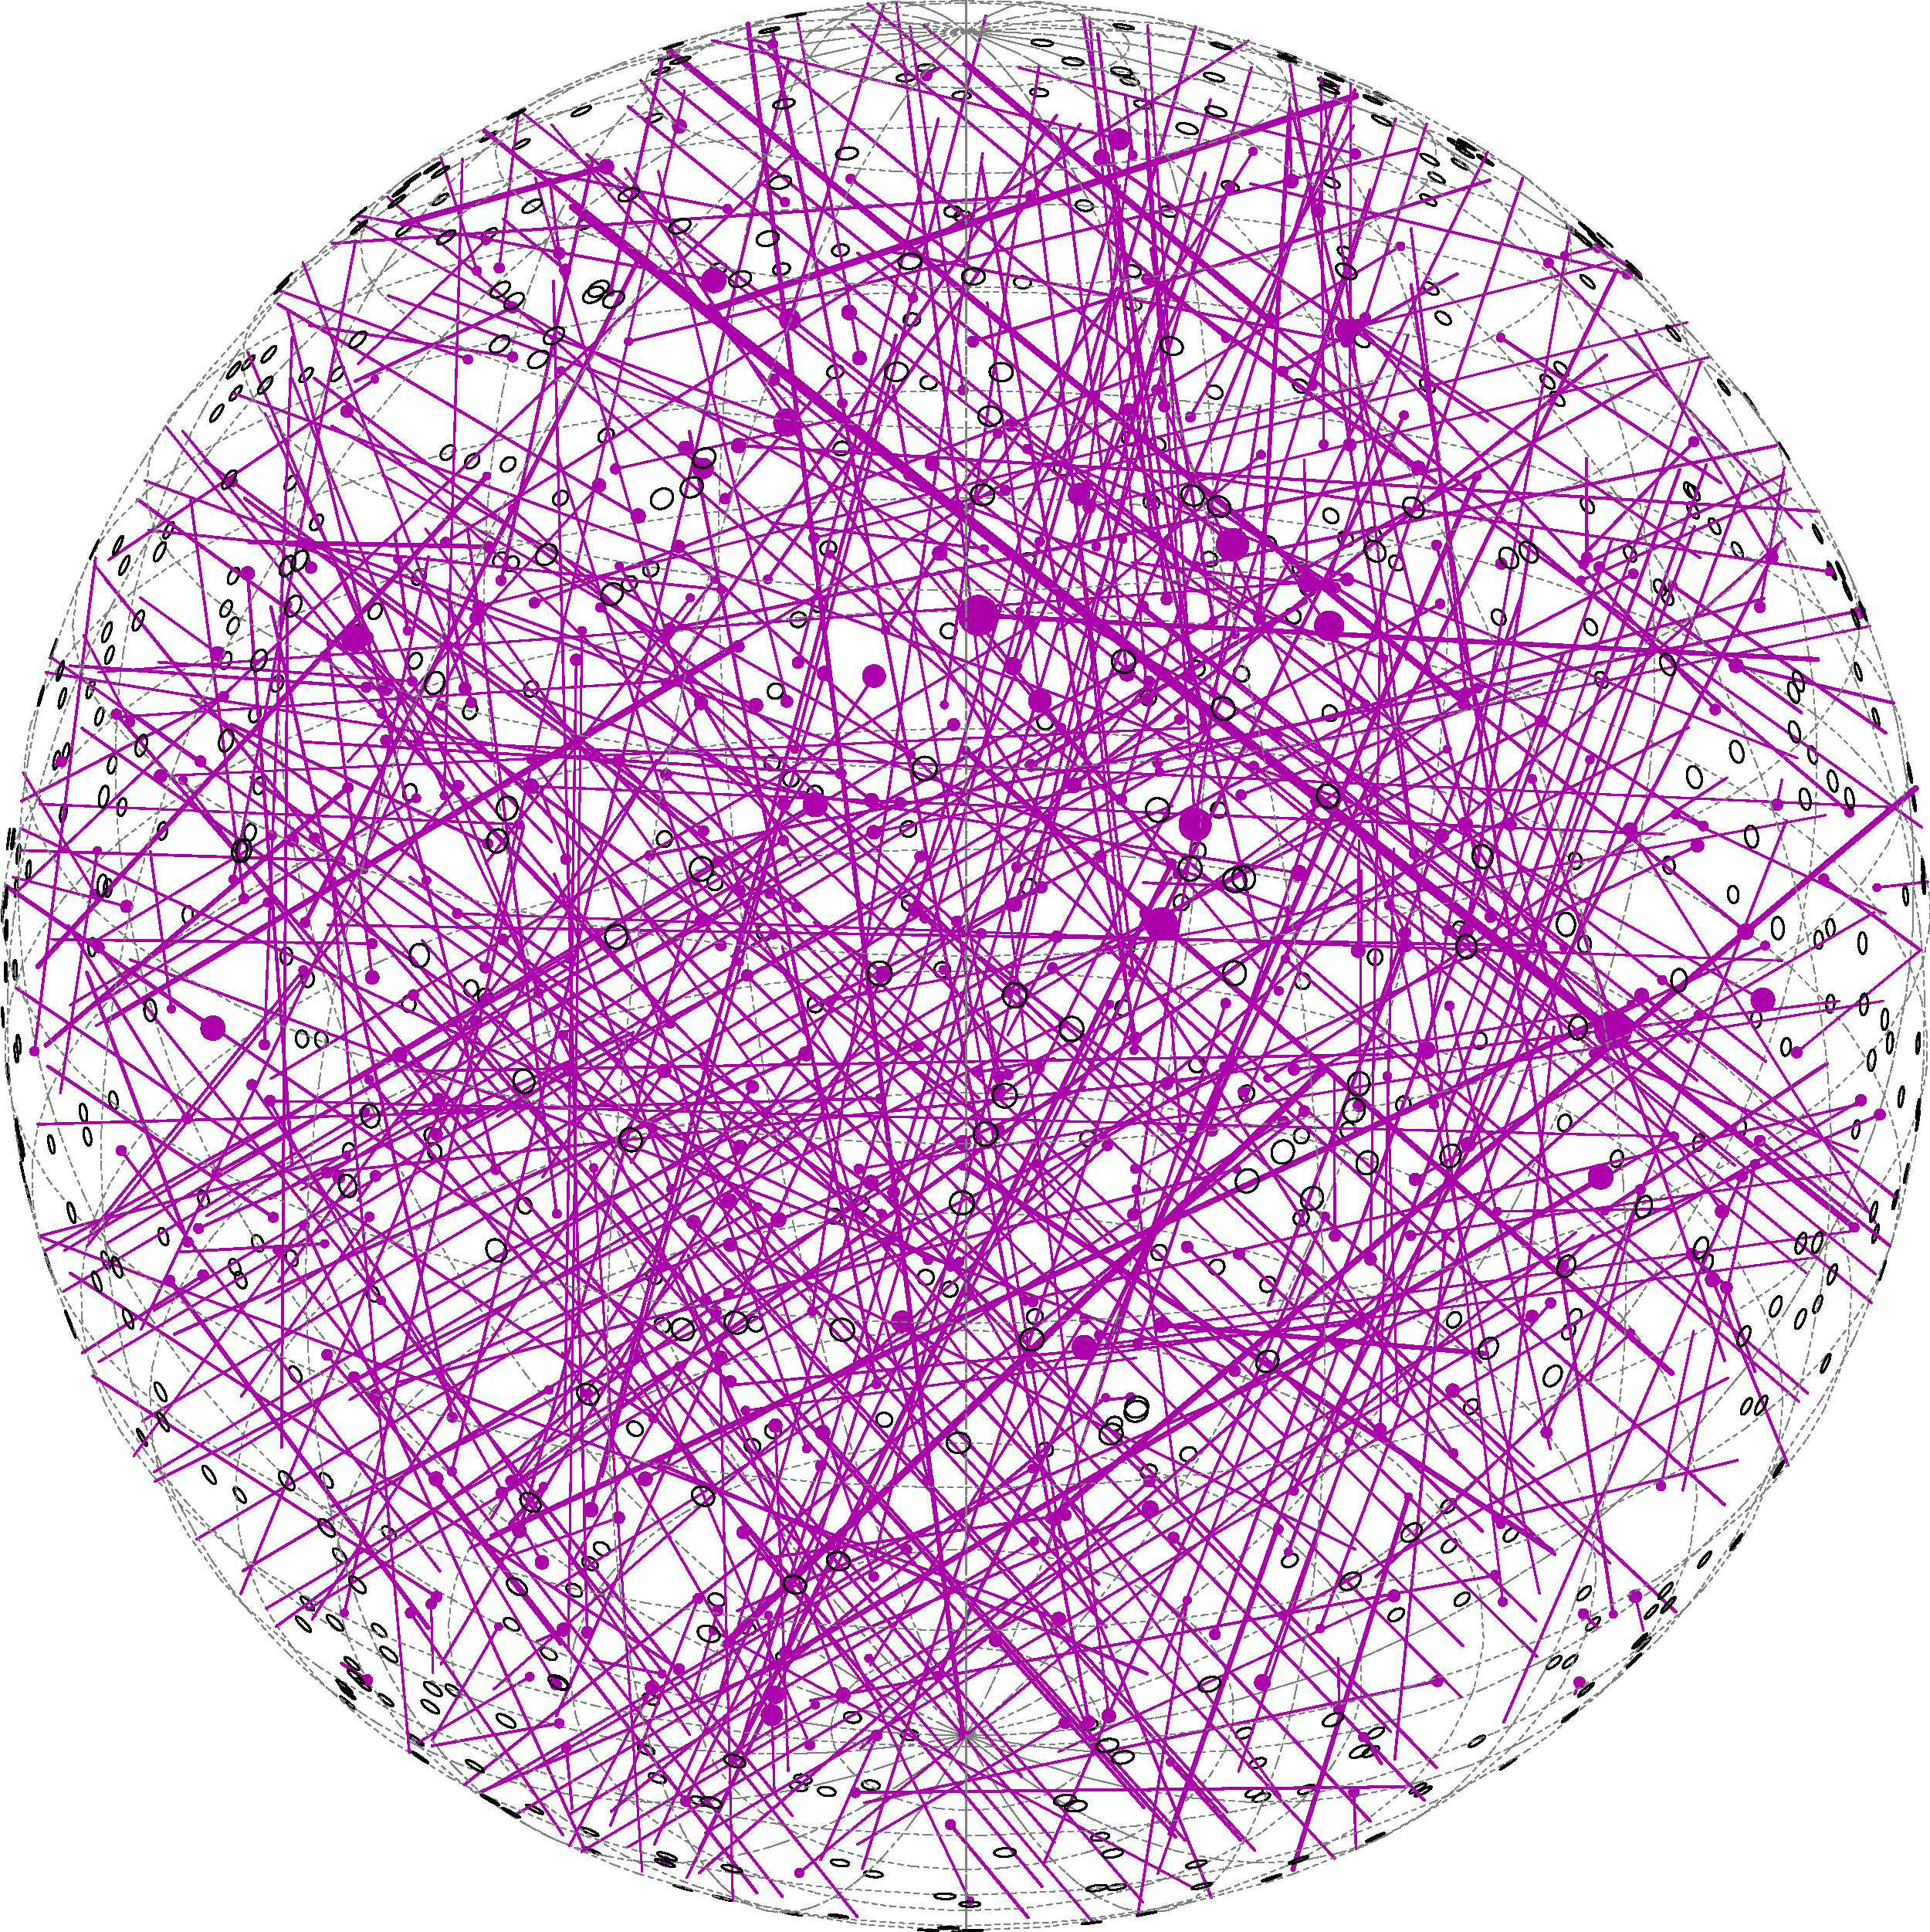
\includegraphics[width=0.45\linewidth,clip=true]{closeview10k-1Mpc}
%\caption{Three-dimensional maps of the space density of SHS with $v_{\infty} > 10^{4}$ km/s. In the left-hand panel is a sphere of radius 20 Mpc, where the paths shown are of SHS that are currently within 1 Mpc of the MW, and the originating primary black holes are shown by the black points. The right-hand panel shows the volume within 1 Mpc of the MW, where the current position of the SHS are denoted with blue points, and their projected positions onto the sky are shown by the open blue circles. Motion of galaxies and cosmological expansion are neglected.}
%\label{fig:map}
%\end{figure*}

\section{Introduction}
Typical stellar velocities throughout the Milky Way are a few hundred km s$^{-1}$. However, there are particular sub-populations of stars that are found to move at greater velocities; these include the hypervelocity stars \citep[$v \lesssim 700$ km/s][]{Brown:2011a}, runaway stars \citep[e.g.][]{Heber:2008a}, and a small fraction of compact objects, with examples being the binary white dwarf LP400-22 \citep[$v > 830$ km s$^{-1}$]{Kilic:2013a} and the kicked pulsar PSR 2224+65 \citep[$\approx 10^{3}$~km~s$^{-1}$,][]{Cordes:1993a}. While these objects are moving quite quickly as compared to most other stars in the galaxy, they still travel at speeds significantly below that observed for stars in our own galactic center, where the velocity of the star with the closet-known approach to the central black hole exceeds \smash{$10^{4}$} km s\smash{$^{-1}$} \citep{Ghez:2005a}, 3\% the speed of light.

In this paper we describe a mechanism by which binary massive black hole (BMBH) mergers can liberate these tightly-bound stars from their host black holes, resulting in semi-relativistic hypervelocity stars (SHS) that are capable of crossing large swaths of the observable universe and hence can serve as a new cosmological messenger. Predicated on numerical calculations of \citet{Sesana:2010a} and \citet{Iwasawa:2011a} that suggest that BMBHs may be excited to very large eccentricities prior to merger, we suggest that many stars originally bound to the less-massive of the two black holes (the secondary) can be ejected in a manner closely resembling the Hills mechanism \citep{Hills:1988a} for the production of hypervelocity stars (HVS). As in the HVS mechanism, these stars can receive a significant speed boost above and beyond their average orbital velocity, occasionally yielding stars with asymptotic velocities $v_{\infty}$ nearing $c$. We demonstrate that no other mechanism aside from eccentric merging BMBHs can accelerate main-sequence stars to speeds in excess of $10^{4}$ km s$^{-1}$, and thus the detection of even a single star moving at a velocity greater than this value would suggest that a significant fraction of BMBH mergers proceed eccentrically. 

\begin{figure}
\centering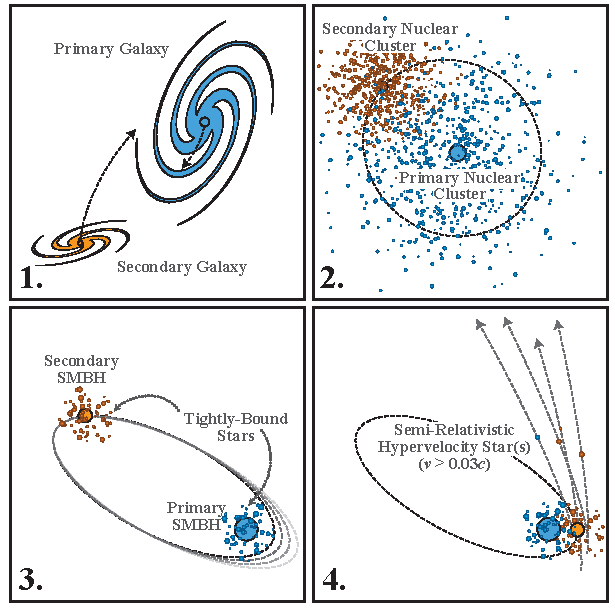
\includegraphics[width=\linewidth,clip=true]{shs-diagram}
\caption{Diagram of primary production channel for SHS. 1: Two galaxies with central black holes merge. 2: Dynamical friction brings the two nuclear clusters and their host MBHs together. 3: The eccentricity of the secondary MBH's orbit about the primary is excited by asymmetrical scattering of stars that originally orbited the primary MBH. A tightly-bound cluster of stars remains bound to the secondary. 4: With each passage of the secondary by the primary, a fraction of stars are ejected as SHS.}
\label{fig:diagram}
\end{figure}

This mechanism is schematically depicted in Figure \ref{fig:diagram}. The merger of two galaxies (panel 1) results in the eventual merger of the nuclear clusters hosting their MBHs (panel 2). As the secondary black hole scatters stars in orbit about the primary, its eccentricity grows quickly to a value of order unity (panel 3). Once the eccentricity has been excited to a large value, the relative binding energy of the secondary to the primary becomes small as compared to the specific binding energy of stars in orbit about either the primary or the secondary, whose eccentricities are on average much lower. As the periapse distance $r_{\rm p,12}$ shrinks, the eccentric Hill radius around the secondary also shrinks, $r_{\rm H,2} = r_{\rm p,12} q_{12}^{-1/3}$, where $q_{12} \equiv M_{1}/M_{2}$, resulting in the removal of all stars with apoapses comparable to this distance (panel 4). In addition to the stars removed from the secondary, stars that are originally in orbit about the primary occasionally enter the secondary's Hill radius. This contributes an additional reservoir of stars that can be accelerated to large velocities, as was demonstrated in \citet{Levin:2006a,Sesana:2006a}.

In this paper we calculate the number of stars accelerated via these two mechanisms, and find that the fastest stars are those that are originally bound to the secondary. To quantify the number of SHS produced by merging BMBHs, we perform Monte Carlo three-body scattering experiments in which random combinations of primary, secondary, and tertiary parameters are drawn, and the outcomes are recorded. We then measure the outgoing velocity of tertiary objects that escape the system and calculate their subsequent evolution from stellar isochrones in order to determine their detectability via current and future surveys. We find that approximately $10^{7}$ objects moving with velocity greater than $10^{4}$ km s$^{-1}$ exist out to the distance of the Virgo cluster ($\sim 10^{3}$ within a Mpc of the MW). Roughly one SHS should be detectable per 10 square degrees for a survey with limiting K-band magnitude of 24, a number that is too small to guarantee a discovery with current surveys, but will yield hundreds of detections with a next-generation all-sky infrared survey such as {\it WFIRST} or {\it Euclid}.

The vast majority of objects that would be detected would be moving slightly faster than $10^{4}$ km s$^{-1}$, with the fastest object that would likely be detected moving at 8\% $c$. Faster objects would exist nearby the Milky Way, but these objects are most likely to be low-mass main-sequence dwarfs that would only be detectable with deep imaging by either {\it HST} or {\it JWST}. Most of the detectable stars will be red supergiants that evolved from stars slightly less than a solar mass, but the Doppler shift associated with such large speeds will make these objects appear significantly bluer than a similar star at rest, with color shifts of greater than half a magnitude in the bluest {\it JWST} bands. Despite their average distance of a Mpc, their large velocities will give them a proper motion that is potentially detectable with {\it LSST} over 10 years.

In Section \ref{sec:speedlimits} we calculate the speed limits for main-sequence stars accelerated via single, double, and triple object mechanisms, and show that only eccentric BMBH mergers can yield main-sequence stars with $v > 10^{4}$ km s$^{-1}$. In Section \ref{sec:experiments} we describe the setup of our numerical scattering experiments, and in Section \ref{sec:results} we describe the outcomes of these experiments. In Section \ref{sec:observations} we calculate the detectability of SHS with various survey constraints. Lastly, we describe the scientific value of SHS if they are detected in Section \ref{sec:discussion}.

\section{Speed Limits of Main-Sequence Stars}\label{sec:speedlimits}
A single star can typically be accelerated to velocities a fraction of its own escape velocity if it can asymmetrically eject a mass comparable to its own mass. Instances of tremendous mass loss usually occur shortly before the birth of a compact object, but mass-loss episodes for stars that do not immediately form compact objects do not result in large bulk velocities for the surviving star. As an example, $\eta$ Carinae, which lost tens of solar masses of ejecta a century ago in an explosive episode, is moving radially towards the Sun at less than 10 km s\smash{$^{-1}$} \citep{Smith:2004a}.

When two objects interact with one another, the maximum velocity in the system is set by the object with the lowest density, as this object determines the minimum approach distance between the two objects before a collision or tidal disruption occurs. If the two objects are point-like and initially bound to one another, the two objects will remain bound indefinitely, assuming Newtonian dynamics. However, there are three possibilities that enable the ejection of an object at a velocity comparable to the maximum orbital velocity of the system: The tidal break-up of one of the two objects, effectively converting the system into a multi-body encounter \citep{Faber:2005a,Manukian:2013a}, the destruction of one of the two stars via a supernova \citep[runaway stars,][]{Blaauw:1961a}, or the tidal break-up of a binary through interaction with a third object \citep{Hills:1988a}.

In the first two cases, the outgoing velocity is limited to a fraction of the velocity at pericenter, which is comparable to the escape velocities from the surfaces of the two objects. In the last case, the outgoing velocity can be enhanced by the presence of the third, more massive object \citep{Hills:1988a}. Because of this additional ingredient, this mechanism can produce stars that are significantly faster than what is possible with a system comprised of only one or two objects.

In the remainder of this section we focus upon the combinations of object types with main-sequence stars and examine the maximum velocities that can be produced for a given combination. Label subscripts for each object are assigned in order of descending mass of the constituents, i.e. ``1'' will always refer to the most massive object in the system (the primary), ``2'' to the second-most massive (the secondary), and ``3'' to the least massive (the tertiary). Double subscripts (e.g. ``12,'' ``23'') refer to quantities that jointly apply to both subscripted objects; as an example $a_{12}$ would refer to the semimajor axis of the primary-secondary system.

\subsection{The Hills Mechanism}

It was found through numerical experiments by \citet{Sari:2010a} that the maximal velocity for an outgoing objects in a Hills encounter ($M_{1} \gg M_{2}$) where $M_{2} = M_{3}$ is
\begin{equation}
v_{\rm kick,\max} = 1.3 v_{23} q_{1,23}^{1/6}\label{eq:vkickmax},
\end{equation}
where $v_{23}$ is the escape velocity from the surface of either the secondary or tertiary object and $q_{1,23} \equiv M_{1}/M_{23}$ ($M_{23} \equiv M_{2} + M_{3}$). This expression can be generalized for the case where $M_{2} \neq M_{3}$ by replacing $v_{23}$ with an expression that accounts for each object's size $R$ and mass $M$,
\begin{equation}
v_{23} = \sqrt{\frac{2 G M_{23}}{R_{2} + R_{3}}}.
\end{equation}
The value in Equation \ref{eq:vkickmax} is typically achieved at a distance $\sim 1/10$ that of the tidal disruption radius of the incoming binary \smash{$r_{\rm t,23} \equiv a_{23} q_{12}^{1/3}$} \citep{Sari:2010a}. Whether this maximum value is realized depends on the initial phase of the binary's orbit, where optimal phases are those in which the secondary and tertiary objects approach each other as closely as possible at the moment of periapse with the primary, without either colliding or tidally disrupting one another. For a maximum kick, the mass ratio $q_{12}$ should be as large as possible, but keeping in mind that $v_{23}$ tends to decrease with increasing $q_{12}$ for a fixed $M_{1}$. The following sections describe how these two scalings compare to one another for specific object types is described in.

\subsubsection{Stellar-Mass Secondaries}
The escape velocity from a main-sequence star scales weakly with stellar mass, as $R_\ast \propto M_\ast^{0.8}$, and thus $v_{\rm esc,\ast} \propto M_\ast^{0.1}$. Because the kick velocity scales as \smash{$q^{1/6} \propto M_{2}^{-1/6}$}, there is no advantage to increasing the mass of the secondary, and in fact the maximum kick velocity {\it decreases} slightly, $v_{\rm kick} \propto M_2^{-0.06}$.

\colr{Move these few sentences to somewhere more logical} This mass ratio can be made arbitrary large so long as the tertiary remains above the hydrogen-burning limit (at $M_{\ast} \sim 13 M_{\rm Jupiter}$), as average stellar density scales inversely with stellar mass, $\bar{\rho} = M_\ast / R_\ast^3 \propto M_\ast^{-1.4}$. Indeed giant planets can be effectively launched at speeds of $\sim 10^{4}$ km/s from our MW's black hole, where $q_{23} \sim 10^{3}$ \citep{Ginsburg:2012a}.

However, increasing $M_{2}$ helps achieve larger kick velocities because only massive star binaries can survive in the nuclear clusters surrounding massive black holes. The mass of the black hole is set by finding the largest black hole that will not swallow the binary whole, i.e. $r_{\rm g} \equiv 2 G M / c^{2} = r_{\rm H}$, where \smash{$r_{\rm H} \equiv (3 q_{1,23})^{1/3} a$} is the disruption radius of the binary. In principle, the binary separation $a_{23}$ can be arbitrarily large and still experience a large kick, provided that the two stars approach one another closely at periapse, but the probability of this occurring for a given passage is progressively smaller for increasing separations. Binaries of separations greater than
\begin{equation}
a_{\max} = \frac{G \left(M_{2} + M_{3}\right)}{\sigma^2},\label{eq:amax}
\end{equation}
where $\sigma$ is the velocity dispersion of the central cluster, are unlikely to survive random encounters with other stars, and thus this sets a limit on the maximum separation. By setting the periapse to $r_{\rm g,1}$ and equating that with the maximal kick periapse ($0.1 r_{\rm H}$) we find that
\begin{equation}
a_{\rm maximal} = 10 \left(\frac{M_2}{M_1}\right)^{1/3} r_{\rm g}\label{eq:amaximal}
\end{equation}

Equating $a_{\max}$ (Equation (\ref{eq:amax})) to $a_{\rm maximal}$ (Equation (\ref{eq:amaximal})) and setting $\sigma$ according to the Faber-Jackson relation ($M_{\rm h} \propto \sigma^{4}$, \citet{Kormendy:2013a}, with $\sigma = \textrm{75 km/s}$ for the Milky Way), we find the primary mass $M_{1}$ that leads to the largest kick given a stellar mass,
\begin{equation}
M_{1,\max} (M_{\ast}) = 6 \times 10^{7} \left(\frac{M_{\ast}}{M_{\odot}}\right)^{4/7} M_{\odot}.
%\left[\frac{c^{12}M_{\rm h,sc}^{3}M_{\ast}^{4}}{4^{7} \times 5^{6} \sigma_{0}^{12}}\right]^{1/7}
\end{equation}
Combing this expression with Equation \ref{eq:vkickmax}, we find the maximal velocity possible for a star of a given mass, independent of $M_{1}$,
\begin{equation}
v_{\rm kick,\max} = \textrm{11,000} \left(\frac{M_{\ast}}{M_{\odot}}\right)^{1/35} \textrm{km/s}\label{eq:vkickmax2},
\end{equation}
which scales extremely weakly with $M_{\ast}$. Any star moving faster than this velocity is very unlikely to be produced by the standard Hills mechanism in which both objects are MS stars, as it would require that a binary with a wide separation with $v_{\rm circ} < \sigma$ passes by the central black hole, which is only possible if the binary is set onto a plunging orbit from beyond the black hole's sphere of influence.

By changing the secondary to a degenerate object, such as a WD or a NS, $M_{2}$ is limited to the Chandrasekhar mass $M_{\rm Ch} \simeq 1.4 M_{\odot}$. This means that either one selects the tertiary to be somewhat less massive than the secondary, or that the compact object becomes the tertiary, limiting the ejection velocity of the (now heavier) MS companion to 0.9 $v_{\rm esc} M_{12}^{1/6}$ \citep{Sari:2010a}. In either case, the maximum kick velocity is smaller than what is possible with two MS stars, whose masses can exceed $M_{\rm Ch}$.

If the secondary is a stellar-mass black hole, $M_{2}$ is not limited by $M_{\rm Ch}$. However, as $r_{\rm g,2} \ll R_{\odot}$ for $M_{2} < 2 \times 10^{5} M_{\odot}$, the separation is still limited by the size of the MS tertiary, and Equation \ref{eq:vkickmax2} again applies.

%\subsubsection{Compact Object Binaries}
%Notes: separation limited by GW merger timescale, except for WD + NS or WD + WD from mass transfer. However, maximum velocities restricted by mergers for these systems.
%\colr{Old stuff}
%\begin{equation}
%F_{\rm ns} F_{\rm bin} F_{\rm ns comp} F_{\rm encounterfrac} \dot{N}_{\rm d} \tau_{\rm H} n_{\rm gal} V
%\end{equation}
%
%Light-speed SHS:
%\begin{align}
%F_{\rm ns} &= 0.001\\
%F_{\rm bin} &= 0.05\\
%F_{\rm ns comp} &= 0.01\\
%F_{\rm encounterfrac} &= 0.01\\
%\dot{N}_{\rm d} &= 10^{-5}\;{\rm yr}
%\end{align}
%10 out to Virgo.\\
%
%1-10\% light-speed SHS:
%\begin{align}
%F_{\rm WD} &= 0.1\\
%F_{\rm bin} &= 0.05\\
%F_{\rm ns comp} &= 0.1\\
%F_{\rm encounterfrac} &= 0.01\\
%\dot{N}_{\rm d} &= 10^{-5}\;{\rm yr}
%\end{align}
%$10^4$ out to Virgo.

\subsubsection{Massive Secondaries}
The only option for secondaries with masses larger than that of the most massive stars ($\sim 300 M_{\odot}$) are black holes. Black hole masses are known to range from a few times solar to tens of billions of solar masses, with a paucity of black holes known to have masses between 100 and $10^{5} M_{\odot}$. If this deficit is real, then it suggests that stars launched via the Hills mechanism have different characteristic velocities. As we showed in the previous section, the limit for main-sequence binaries is $\sim 11,000$ km/s, but this limit arises from the fact that main-sequence stars of increasing mass have increasing size, and thus collide rather than resulting in an ejection. Black holes do not have this limitation, so in principle the maximum velocity possible for a non-spinning black hole is given by the velocity at the Schwarzschild radius of the secondary $r_{\rm g,2}$: The speed of light $c$.

The picture is of course complicated by general relativity, which can cause particles on orbits of finite energy to inspiral exterior to $r_{\rm g}$, depending on the black hole's spin. As a hypervelocity ejection is typically the result of the tertiary being placed on a near-radial orbit about the secondary by the primary, it approaches the secondary on a parabolic orbit, which would inspiral into the secondary at its IBCO at $2 r_{\rm g,2}$ for a non-spinning black hole. As a result, the maximum possible velocity is set at this distance rather than $r_{\rm g}$. This suggests that the speed limit for semi-relativistic hypervelocity stars (SHS) is $c/2$ (including the relativistic boost factor $\gamma$), and possibly more for spinning black holes, which we do not consider here.

This speed is a factor of $\sim 15$ times larger than the speed limit for main-sequence star binaries. If the spectrum of SHS velocities were similar to that of HVS, in which the typical velocities are a few thousand km/s, it would suggest that the average SHS's speed is a few ten thousands km/s. However, two important factors influence the SHS velocity distribution: The secondary's binding energy to the primary, which determines the depth of the potential well that any ejected tertiary would need to climb out of, and the distribution of orbits about the secondary, which is quite different from the distribution of orbits of stellar binaries.

\subsection{Importance of Secondary's Orbital Energy}
For the traditional HVS mechanism, the incoming binaries are deposited into the loss cone via kicks they receive typically near apoapse, and the majority of these binaries originate from the primary's sphere of influence \colr{cite}. At this distance, the binding energy to the black hole is small ($\sim \sigma^{2}$), and thus the kick received by an ejected star is only reduced by a small amount.

For the SHS mechanism, the secondary's orbital energy depends entirely on how the two black hole clusters merge. The traditional picture has been that dynamical friction drags the secondary black hole and its surrounding stars into the outskirts of the primary's nuclear cluster. At this point, stars are scattered by the secondary with no preferred direction, resulting in an inspiral in which the secondary's orbit remains approximately circular at all times. This means that stars that are tidally removed from the secondary by the primary will only leave with a velocity comparable to the local velocity dispersion, and will not escape the primary's gravity.

However, numerical $N$-body results \citep{Iwasawa:2011a,Khan:2012a} suggest that the secondary's orbit does not remain circular during its inspiral owing to a preferential ejection of stars orbiting the primary in the same direction as the secondary. They suggest that the orbit can become extremely eccentric, with $e \sim 0.999$ for $M_{1} = 10^{10} M_{\odot}$ and $M_{2} = 10^{8} M_{\odot}$. The authors suggest that the only mechanism that prevents a total plunge ($e = 1$) is the random noise introduced by the discrete nature of the scattered stars, which suggests that more massive primaries would result in even more extreme maximum eccentricities. If such behavior occurs in nature, the specific orbital energy of the secondary black hole is comparable to that of incoming stellar binaries in the HVS scenario, and thus the velocities of ejected stars will not be reduced much by their initial orbital energy.

We conclude that an eccentric secondary is absolutely required for the production of SHS: If the incoming secondary's orbit remains circular at all times, SHS will not be produced. Because SHS are not capable of being produced by any other known astrophysical mechanism, this means that the detection of SHS would strongly suggest that at least some fraction of BMBH merge eccentrically.

\section{Rates}

\subsection{Loss-Cone Filling by Marginally Bound Stars}

\colr{Here we talk about the Alberto Sesana and Qingjuan Yu method for producing stars. Talk about how stars can occupy energies $< G M_{\ast}/R_{\ast}$ \citep[response to][]{Yu:2003a}.}

\subsection{Removal of Secondary's Cluster}
In the initial stages of a merger, the secondary retains a retinue of stars within its Hill radius, whose distribution likely resembles the original distribution of stars. Prior to merger, the radial distribution of these stars likely resembles $n(r) \propto r^{-7/4}$ \citep{Bahcall:1976a} exterior to the distance where the orbital velocity $v_{\rm orb} = \sqrt{G M_{2} / r}$ is less than the escape velocities from typical stars, $v_{\ast} = \sqrt{G M_{\ast} / R_{\ast}}$. If the black hole is surrounded by a population of stellar mass black holes, this distribution can continue a factor of a few more in $r$ before terminating, as stars would be capable of relaxing to higher binding energies without colliding \citep{OLeary:2008a}. In such systems, $N(a) \propto a^{1/4} e$ \citep{Merritt:2013a}. However, if we consider a scenario where the cluster orbits within a larger cluster on an eccentric orbit, the boundary condition of the secondary's cluster is complicated. Not only does the region within which the secondary dominates the dynamics change in size, the conditions at its boundary change with distance from the central black hole.

If we presume that the cusp of stars around the primary follows a power-law distribution with $r$, $\rho \propto r^{-\alpha}$, then the stalling radius is given by the distance within which a mass $M_{2}$ of stars is contained ,
\begin{equation}
a_{\rm s} = a_{\rm h} q^{\frac{1}{3-\alpha}},
\label{eq:astall}
\end{equation}
where $a_{\rm h}$ is the sphere of influence radius of the primary. At this distance, the stellar density is
\begin{equation}
\rho(a_{\rm s}) = \frac{3 \left(\alpha - 3\right)}{4 \pi} \left(\frac{M_{2}}{M_{1}}\right)^{\frac{\alpha}{\alpha - 3}} \frac{M_{1}}{a_{\rm h}^{3}}.
\label{eq:rhostall}
\end{equation}

At the primary's sphere of influence, the velocity dispersion is
\begin{equation}
\sigma_{1} = 75 \left(\frac{M_{1}}{4 \times 10^{6} M_{\odot}}\right)^{0.25} \textrm{km}\label{eq:sigma},
\end{equation}
the Hill radius at this location is
\begin{equation}
r_{\rm H} = \left(\frac{M_{1}}{3 M_{2}}\right)^{1/3} \frac{G M_{1}}{\sigma_{1}^{2}}.
\end{equation}
%If we now consider the sphere of influence of the secondary, we find that it is always smaller than the Hill radius by a factor $(M_{1}/M_{2})^{0.17}$, this suggests that most stars that are originally bound to the secondary will remain bound to it at the initial phase of the inspiral.

As the secondary's eccentricity grows, the Hill radius shrinks as the secondary's periapse comes closer to the primary. This results in the stripping of the outermost stars in orbit about the secondary. As the eccentric growth rate is slow \citep[$\sim 10^{8}$ yr,][]{Iwasawa:2011a}, stars are almost always removed when their apoapse is larger than secondary's eccentric Hill sphere at periapse,
\begin{equation}
r_{\rm H,e} = (1 - e_{12}) r_{\rm H}.
\end{equation}
This means that stars with the smallest separations from the secondary are removed in the final phases of the secondary's inspiral, these stars are the ones that potentially have the largest ejection velocities, so long as the secondary's orbit remains eccentric during the inspiral. Eventually, every single star that was once bound to the secondary will experience one of the following outcomes: Become bound to the primary, be swallowed or tidally disrupted by one of the two black holes, or become unbound to both the primary and the secondary. This last possibility is what can potentially produce SHS.

\subsubsection{Justification for single-scattering approximation}
\colr{The following is new and out of order with the rest of the paper.} In the three-body scattering experiments presented thus far, the majority of our calculations have only been over a single orbit, where we selected a particular distance interior to the secondary-tertiary Hill radius. However, the secondary black hole's eccentricity increases slowly as a function of time, meaning that the secondary-tertiary system gradually becomes more and more prone to perturbation from the primary. In principle, the tertiary can be lost well before $a_{23} > r_{{\rm H},23}$, meaning that the maximum kick velocity is severely limited \citep{Sari:2010a}.

\begin{figure}
\centering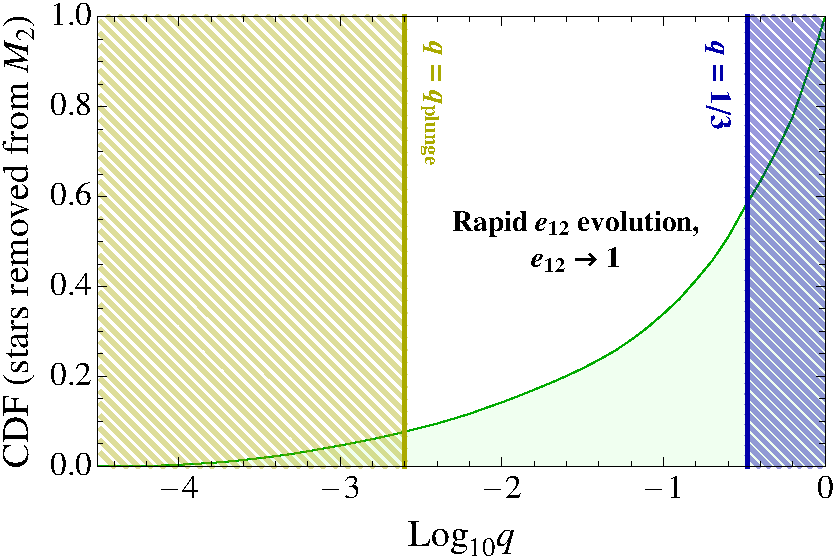
\includegraphics[width=\linewidth,clip=true]{qplunge}
\caption{Cumulative distribution function of hypervelocity stars produced from mergers of a given $q$. Below a critical mass ratio $q_{\rm plunge}$ (Equation~(\ref{eq:qplunge})), the cross-section of the secondary is small, reducing its dynamical drag and rate of eccentricity excitation \citep{Iwasawa:2011a}. Above $q_{\rm plunge}$, the secondary's eccentricity evolves on a timescale comparable to an orbital period. For $q \gtrsim 1/3$ (A. Sesana, priv. comm.), eccentricity excitation ceases to be effective, as both black holes begin to orbit a common center of mass.}
\label{fig:qplunge}
\end{figure}

\citet{Iwasawa:2011a} presented an expression for the eccentricity growth timescale $T_{e}$ as a function of the primary-secondary binary parameters, which we reproduce here using our notational conventions,
\begin{align}
T_{e} &\sim 1.4 \times 10^{8} \left(\frac{M_{1}}{10^{10} M_{\odot}}\right)^{3/2}\left(\frac{M_{\rm s}}{10^{8} M_{\odot}}\right)^{-1}\nonumber\\
&\times \left(\frac{a}{10\;{\rm pc}}\right)^{-3/2}\left(\frac{\rho}{100 M_{\odot}\;{\rm pc}^{-3}}\right)^{-1} {\rm yr}.
\label{eq:te}
\end{align}
The main uncertainty in this equation are what values to assign to $a$ and $\rho$. When two central black holes merge, their evolution is initially governed by dynamical friction, which causes the light of the two black holes to sink rapidly towards the heavier \citep{Dotti:2012a}. During this phase, the orbit remains fairly circular. This phase ceases once the secondary black hole reaches a distance from the primary within which $\sim 2 M_{2}$ worth of stars lies within $a$ \citep{Matsubayashi:2007a}, at which point $a$ ceases to evolve for isotropic stellar distributions. At this point, the eccentricity of the secondary begins to grow, and thus the values of $a$ and $\rho$ chosen should be selected at the stalling radius of the secondary $a_{\rm s}$.

Setting $a = a_{\rm s}$ (Equation \ref{eq:astall}) and $\rho = \rho(a_{\rm s})$ (Equation \ref{eq:rhostall}) in Equation (\ref{eq:te}) and taking the ratio of this timescale to the secondary's orbital period at $a_{\rm s}$, we find
\begin{equation}
\frac{T_{e}}{P} = \frac{5.6 \times 10^{-3}}{3 - \alpha} \frac{\sqrt{1 + q}}{q^{2}},
\end{equation}
where $q \equiv M_{2}/M_{1}$. Setting $T_{e}/P = 1$, assuming $q \gg 1$, and solving for $q$ we find the critical mass ratio necessary for rapid eccentricity evolution $q_{\rm plunge}$,
\begin{equation}
q_{\rm plunge} \simeq \frac{0.03}{\left(3 - \alpha\right)^{2/3}} \label{eq:qplunge}
\end{equation}
However, it has been shown that near-equal mass MBHs ($q \gtrsim 1/3$) do not show strong eccentricity growth \citep{Sesana:2010a} \colr{Try to find more citations here}. As $T_{e}/P$ increases with decreasing $q$, this suggests that there must be a critical $q$ value for which eccentricity excitation is the most effective.

\subsection{Capture and Ejection of Primary Binaries}

After these stars have been exhausted, new stars must be acquired to continue producing SHS. One possible channel is the capture of stellar binaries that originally orbited the primary. The capture cross-section is
\begin{equation}
P(< b) = b^2 \left[1 + \left(\frac{v_{\rm esc,2}}{v_{\rm c,1}}\right)^2 \right]
\end{equation}
The majority of captures are marginally gravitationally focused as $v_{\rm esc,2} = v_{\rm c,1} q_{12}^{-1/3}$, however deeper encounters will experience significant gravitational focusing.

\section{BMBH Scattering Experiments}\label{sec:experiments}
To determine the rate of stellar ejections, we perform Monte Carlo scattering experiments using the same orbit integration routines in {\tt Mathematica} (version 9.0) of \citet{Manukian:2013a} used to investigate the production of ``turbovelocity'' stars. While this approach is only modestly scalable to multiple processors on a single machine, it has the advantage of completely controllable numerical errors, at the expense of increased computational cost. For this paper we perform the calculations in quadruple precision, and restrict the maximum error in the orbital energy and elements of the angular momentum to a part in $10^{30}$.

The parameter space to be explored is quite large; MBHs range over five orders of magnitude in mass, and the stars that orbit them possess a range of masses and orbital parameters. Additionally, the rate of binary massive black hole (BMBH) mergers is very poorly quantified, especially for those black holes that are separated by less than 1 kpc, which are difficult to resolve observationally \colr{add references from deane 2014}.

To better constrain the available parameter space, we consider which sorts of black hole mergers (presuming eccentric mergers are ubiquitous) would give us the highest number of ejected stars with velocities in excess of 10,000 km/s. Because the velocity is set by the minimum approach distance, we wish that the secondary does not tidally disrupt the ejected star where the circular velocity is equal to this value,
\begin{equation}
t
\end{equation}

\section{Results}\label{sec:results}

\begin{figure}
\centering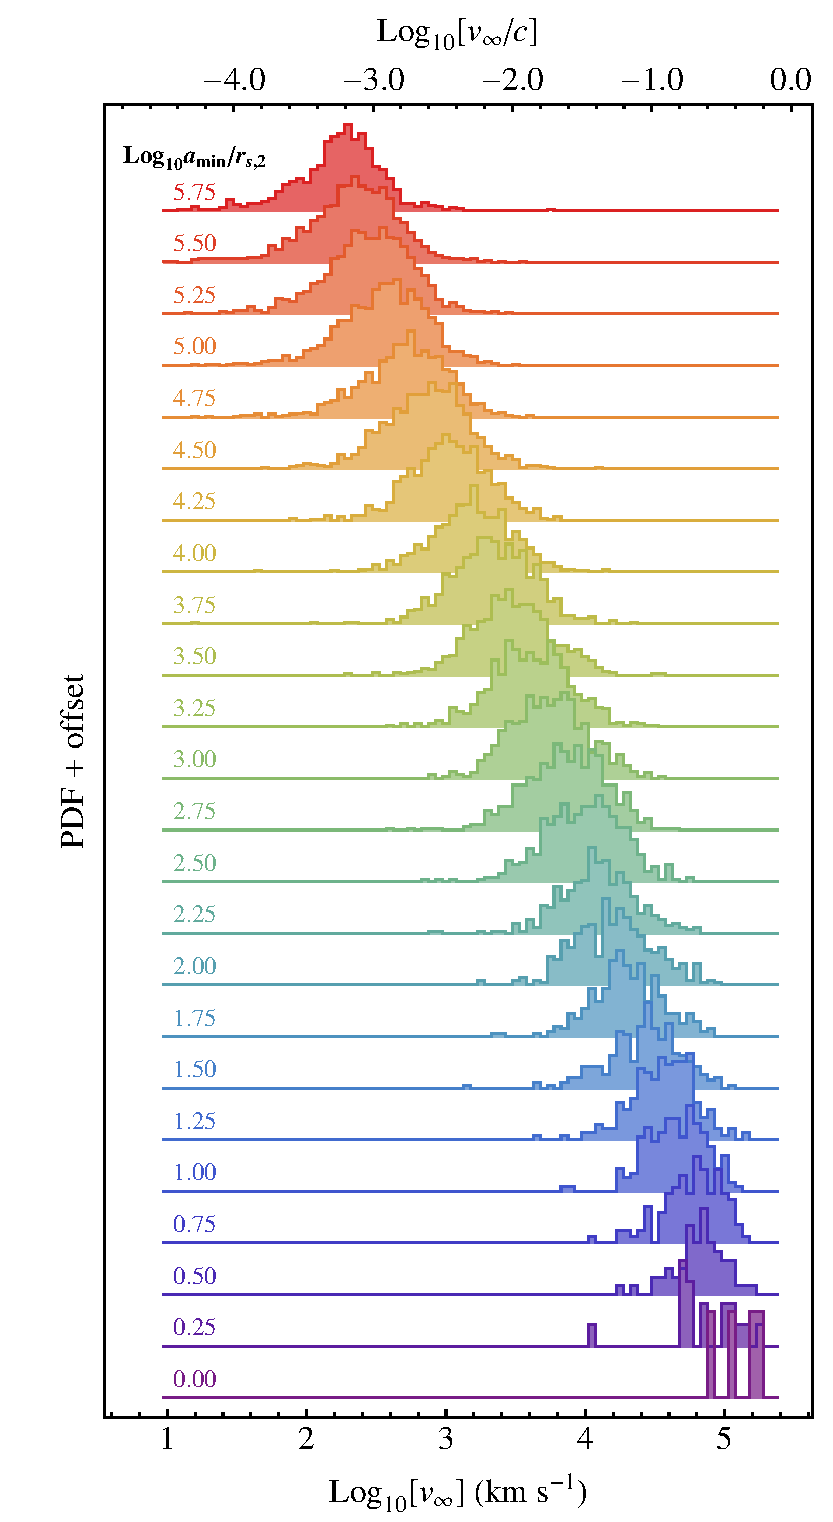
\includegraphics[width=0.9\linewidth,clip=true]{vinfPDF}
\caption{Probability distribution functions of the asymptotic velocity $v_{\infty}$ of stars ejected from merging BMBHs. Each histogram shows the outcome of a set of scattering experiments for a restricted range of initial semimajor axes of the tertiary about the secondary, $a_{\min} < a_{23} < a_{\max}$, where $a_{\min}$ and $a_{\max}$ are spaced logarithmically in intervals of 0.25, with purple corresponding to $a_{\min} = r_{\rm s,2}$ and red corresponding to \smash{$a_{\max} = 10^{6} r_{\rm s,2}$}. Each histogram shows the results of an independent scattering experiment composed of 4,096 systems, where the parameter combinations are drawn as described in Section \ref{sec:experiments}, and are plotted normalized to the bin with the most systems within each histogram.}
\label{fig:vinfpdf}
\end{figure}

\begin{figure}
\centering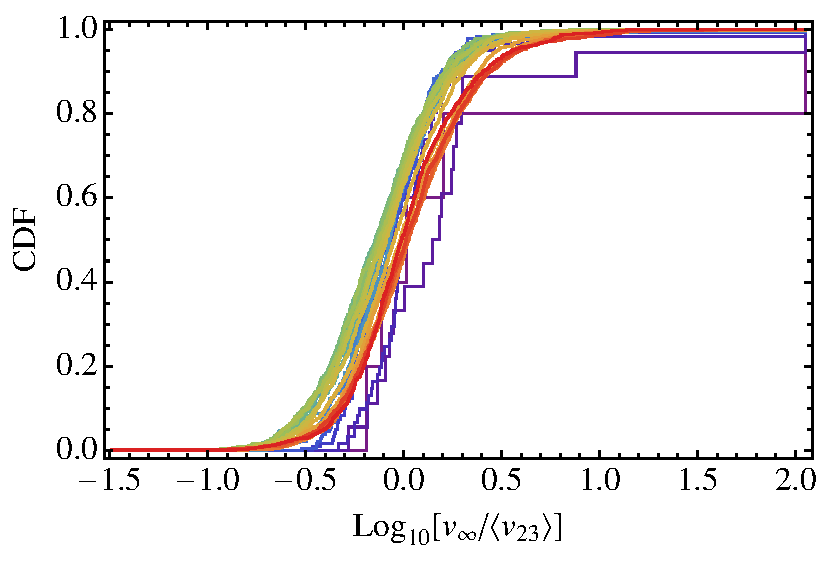
\includegraphics[width=0.9\linewidth,clip=true]{vratio}
\caption{Cumulative distribution functions of the ratio of $v_{\infty}$ to the average velocity of the star's orbit about the secondary prior to its ejection, $\left<v_{23}\right>$. Each CDF is color-coded to the particular scattering experiment labeled in Figure \ref{fig:vinfpdf}.}
\label{fig:vratio}
\end{figure}

\begin{figure*}
\centering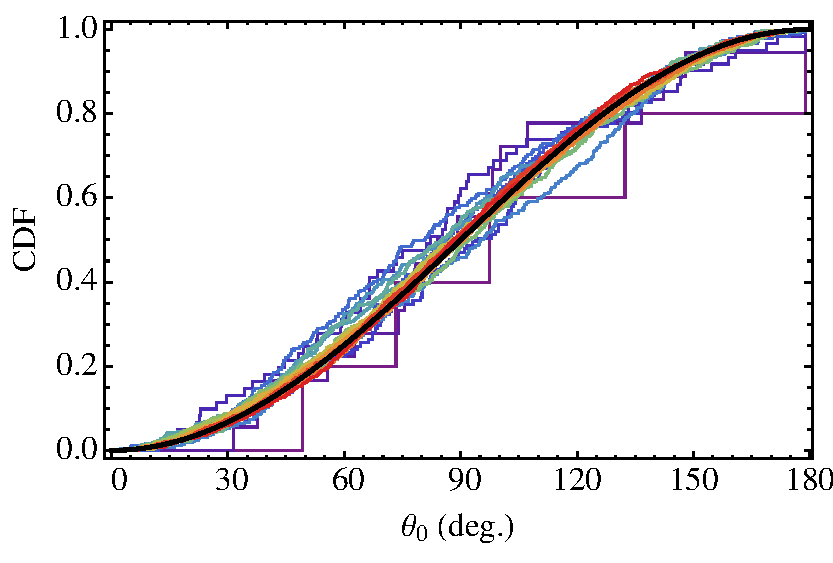
\includegraphics[width=0.45\linewidth,clip=true]{thetaCDF}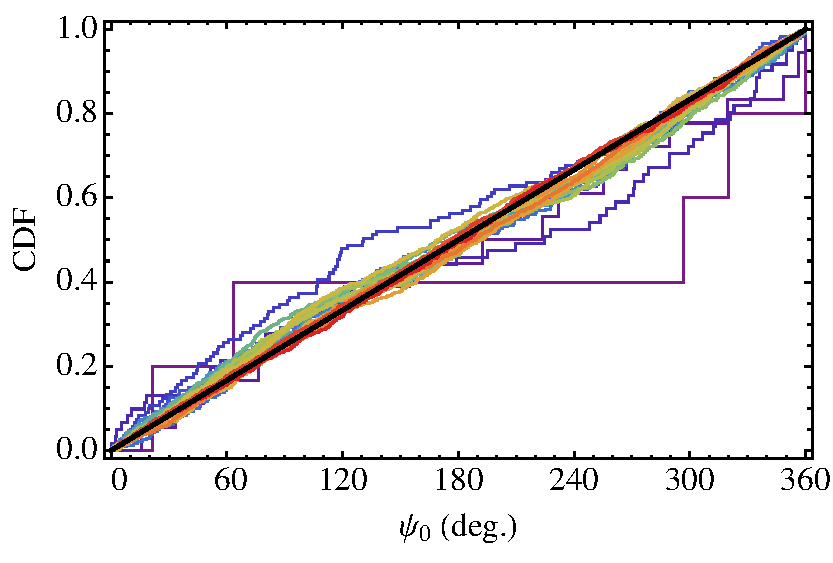
\includegraphics[width=0.45\linewidth,clip=true]{psiCDF}\\
\centering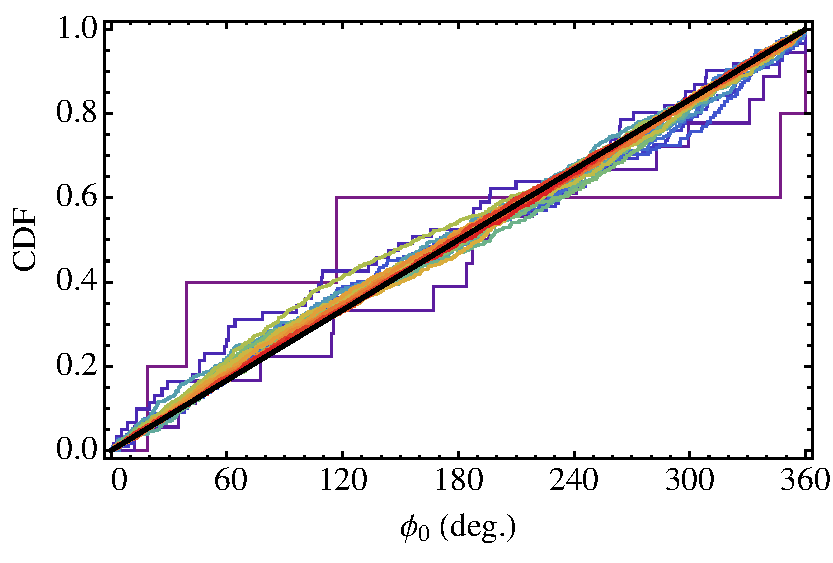
\includegraphics[width=0.45\linewidth,clip=true]{phiCDF}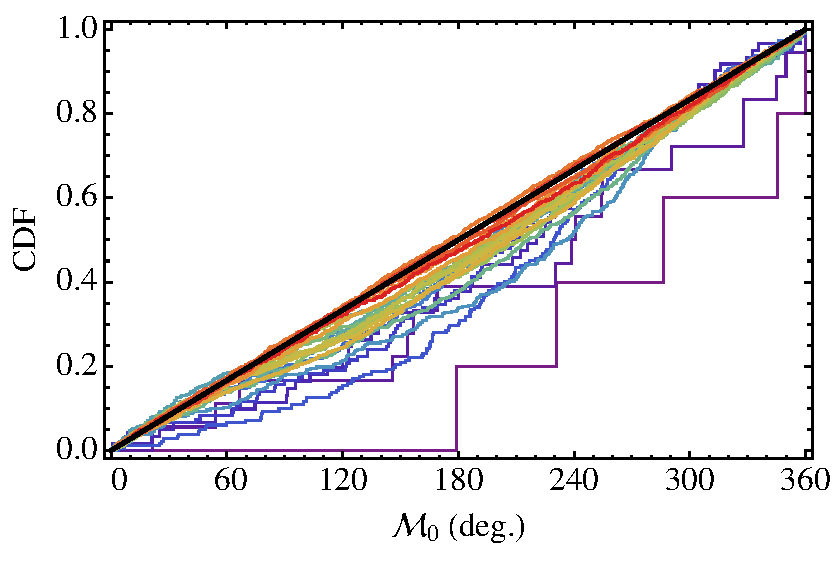
\includegraphics[width=0.45\linewidth,clip=true]{MCDF}
\caption{Cumulative distribution functions of the initial orientation ($\theta_{0}$, $\psi_{0}$, $\phi_{0}$) and mean anomaly ${\cal M}_{0}$ of stars that wound up being ejected from their BMBH system. Each CDF is color-coded to the particular scattering experiment labeled in Figure \ref{fig:vinfpdf}. The thick black curves shows the input distributions assumed for each variable, and are uniform for $\phi_{0}$, $\psi_{0}$, and ${\cal M}_{0}$, and distributed as \smash{$\sin^{2} \theta_{0}$} for the azimuthal angle $\theta_{0}$.}
\label{fig:angle0}
\end{figure*}

\begin{figure*}
\begin{minipage}[b]{0.5\linewidth}
\centering
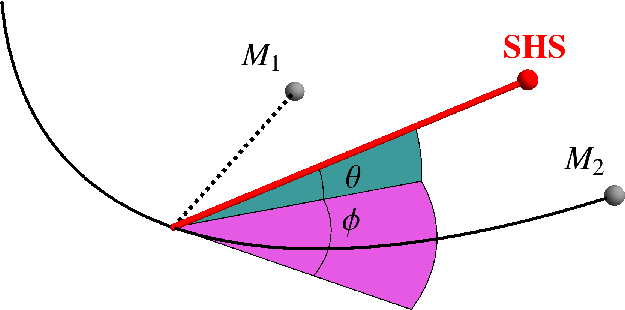
\includegraphics[width=0.8\linewidth,clip=true]{angles-diagram}\\
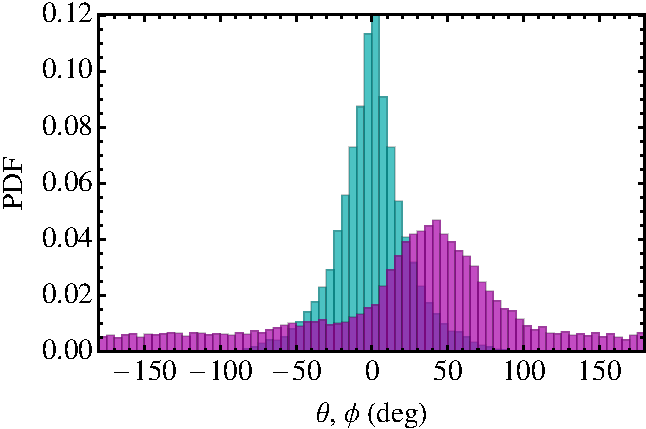
\includegraphics[width=0.8\linewidth,clip=true]{angles-hist}
\end{minipage}
\begin{minipage}[b]{0.5\linewidth}
\centering
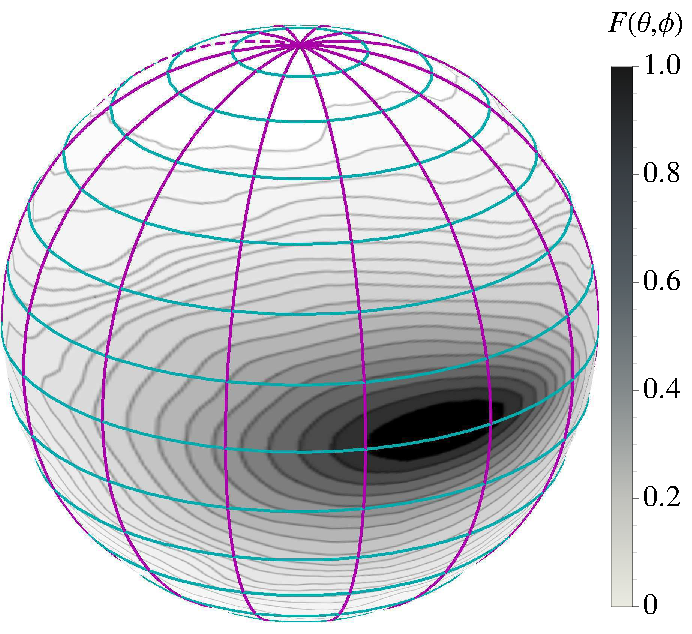
\includegraphics[width=\linewidth,clip=true]{angles-2d}
\end{minipage}
\caption{Distribution of velocity vector angles for SHS. Cumulative fraction $F(\theta, \phi)$ of ejected stars with $v_{\infty} > 0$. The diagram in the upper left shows the positions of the three objects (primary black hole, labeled $M_{1}$, secondary black hole, labeled $M_{2}$, and tertiary star, labeled SHS) shortly after the ejection of an SHS, where $\phi$ is the polar angle and $\phi = 0$ is defined to be the angle of $M_{2}$'s velocity vector at periapse, and the azimuthal angle $\theta$ is measured from the orbital plane. The single-parameter histograms in the bottom-left panel and the 2D histogram mapped to the surface of a sphere show that SHS are preferentially "beamed" in a cone centered at $\theta = \pi/4$ and $\phi = 0$ \citep[see][]{Sesana:2007a,Zier:2001a}.}
\label{fig:ejangles}
\end{figure*}

\begin{figure}
\centering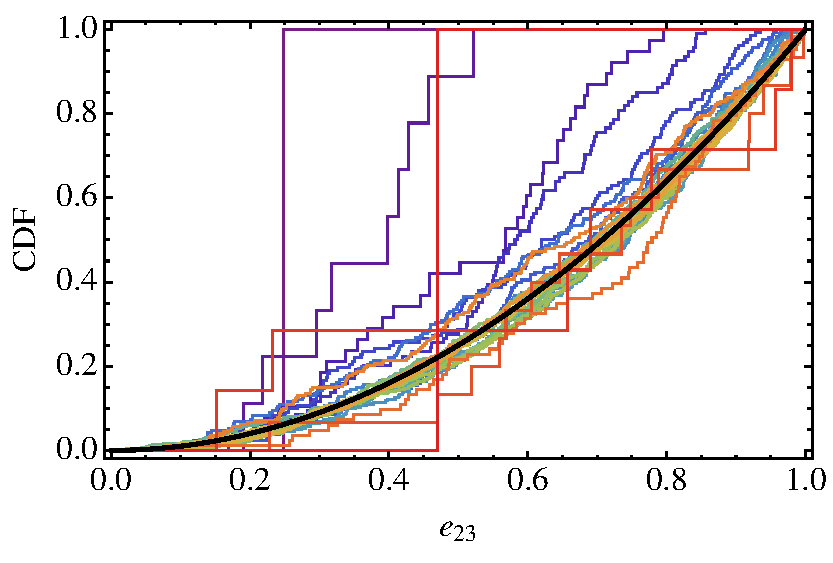
\includegraphics[width=0.9\linewidth,clip=true]{eCDF}
\caption{Cumulative distribution function of the initial eccentricity of the star about the secondary $e_{23}$. Each CDF is color-coded to the particular scattering experiment labeled in Figure \ref{fig:vinfpdf}, and the thick black curve shows the initially assumed thermal distribution, $P(e) \propto e$.}
\label{fig:ecdf}
\end{figure}

\begin{figure}
\centering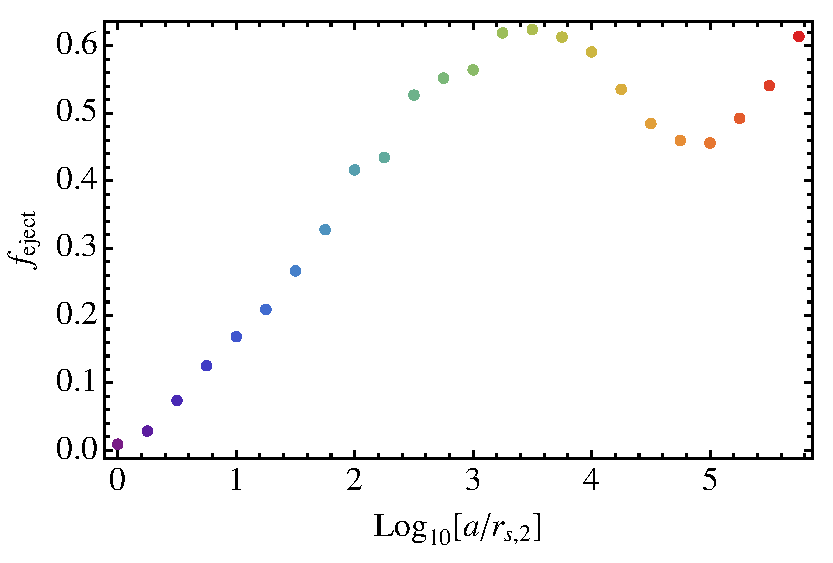
\includegraphics[width=0.9\linewidth,clip=true]{feject}
\caption{Fraction of stars $f_{\rm eject}$ that are ultimately ejected from their host BMBH as HVS. Each point is color-coded to the particular scattering experiment labeled in Figure \ref{fig:vinfpdf}, where the $a$ shown corresponds to $a_{\min}$. At increasing separations, a larger fraction of stars are ejected as HVS, until the separation between the star and the secondary becomes comparable to the secondary's sphere of influence, at which point $f_{\rm eject}$ decreases as $e_{12}$ approaches zero.}
\label{fig:feject}
\end{figure}

\begin{figure*}
\centering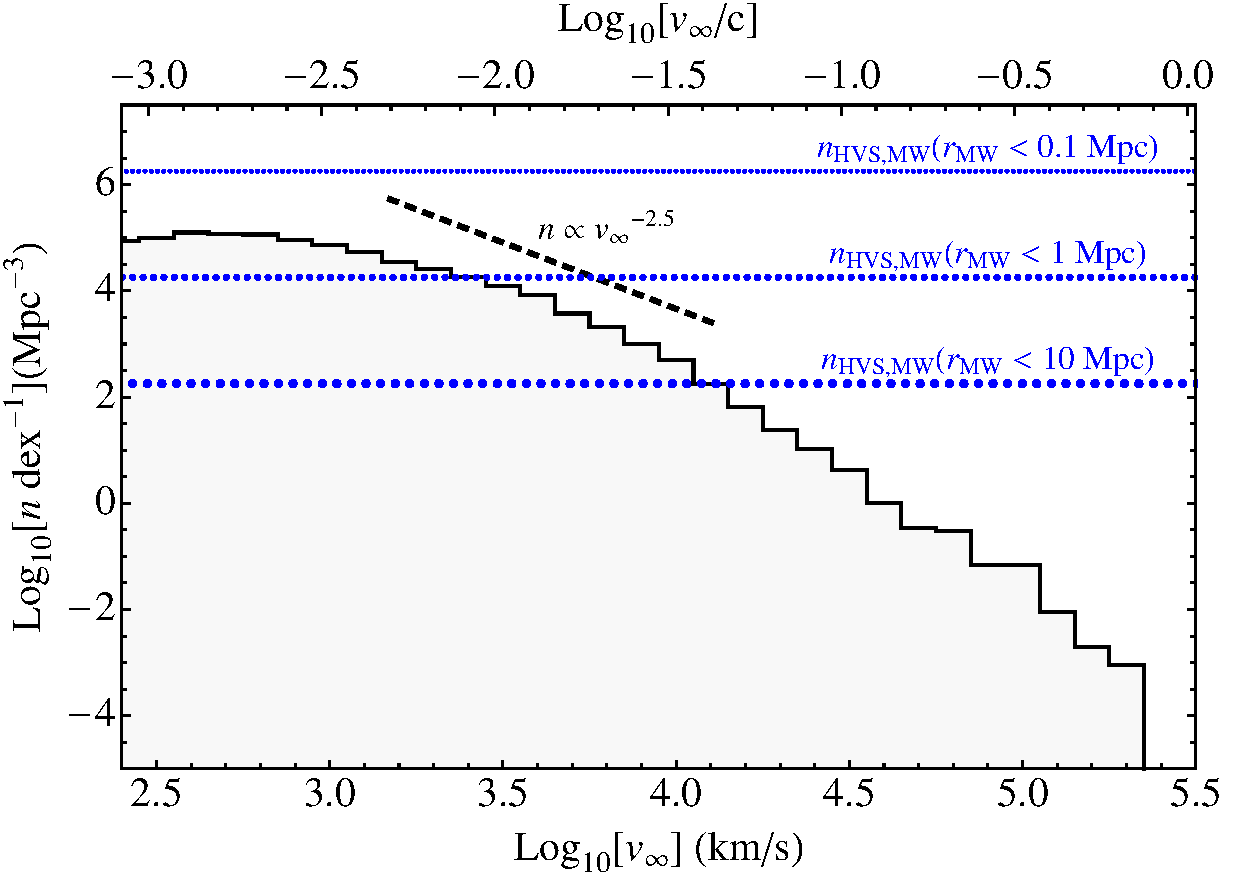
\includegraphics[width=0.7\linewidth,clip=true]{histogram}
\caption{Volume density $n$ as a function of velocity at infinite distance from the binary MBH $v_{\infty}$ of SHS when host galaxy potentials are ignored. The light gray curves show the outcome of each scattering experiment, where the histograms have been properly normalized to account for the different numbers of systems within each $a$ bin. The thick black curve shows the cumulative histogram resulting from the weighted addition of all the individual scattering experiments. The two dotted line segments show the two power-laws expected...}
\label{fig:histogram}
\end{figure*}

\begin{figure*}
\centering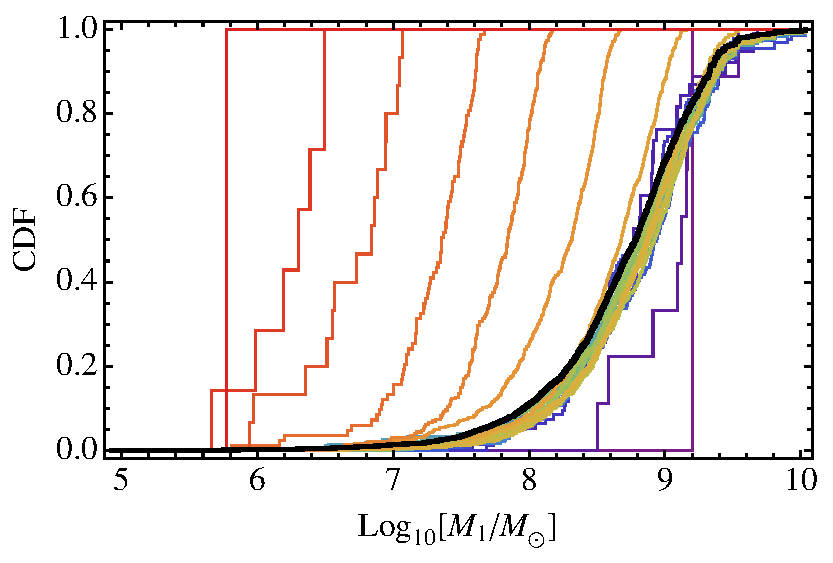
\includegraphics[width=0.45\linewidth,clip=true]{m1CDF}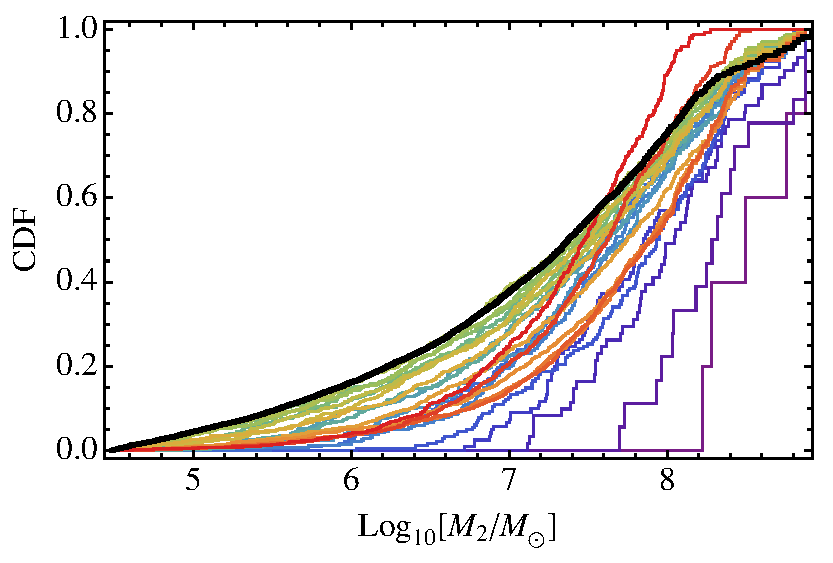
\includegraphics[width=0.45\linewidth,clip=true]{m2CDF}\\
\centering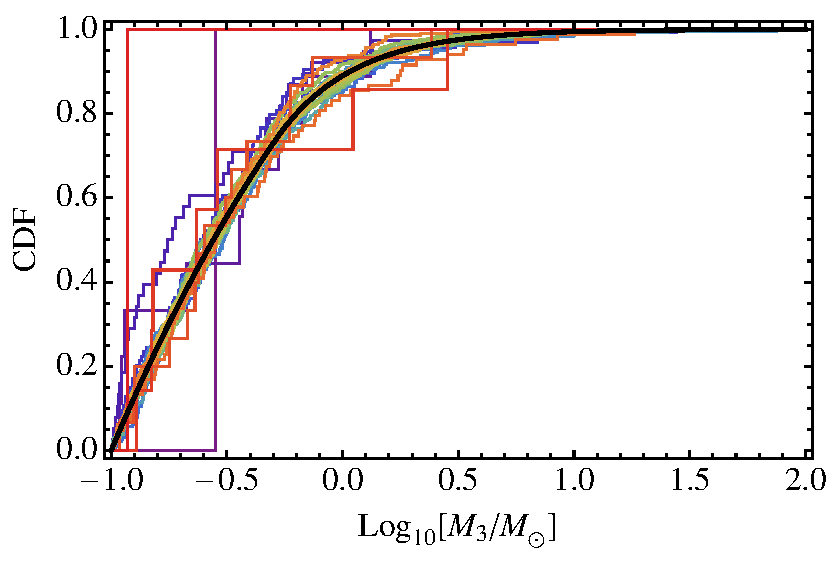
\includegraphics[width=0.45\linewidth,clip=true]{m3CDF}\includegraphics[width=0.45\linewidth,clip=true]{qCDF}
\caption{Cumulative distribution functions of the primary, secondary, and tertiary masses, and the ratio of the secondary to the primary mass $1/q_{12}$. Each CDF is color-coded to the particular scattering experiment labeled in Figure \ref{fig:vinfpdf}. The thick black curve in each panel shows the initially assumed distributions for each mass, as described in Section \ref{sec:experiments}.}
\label{fig:mcdf}
\end{figure*}

\section{Observations}\label{sec:observations}

\begin{figure*}
\centering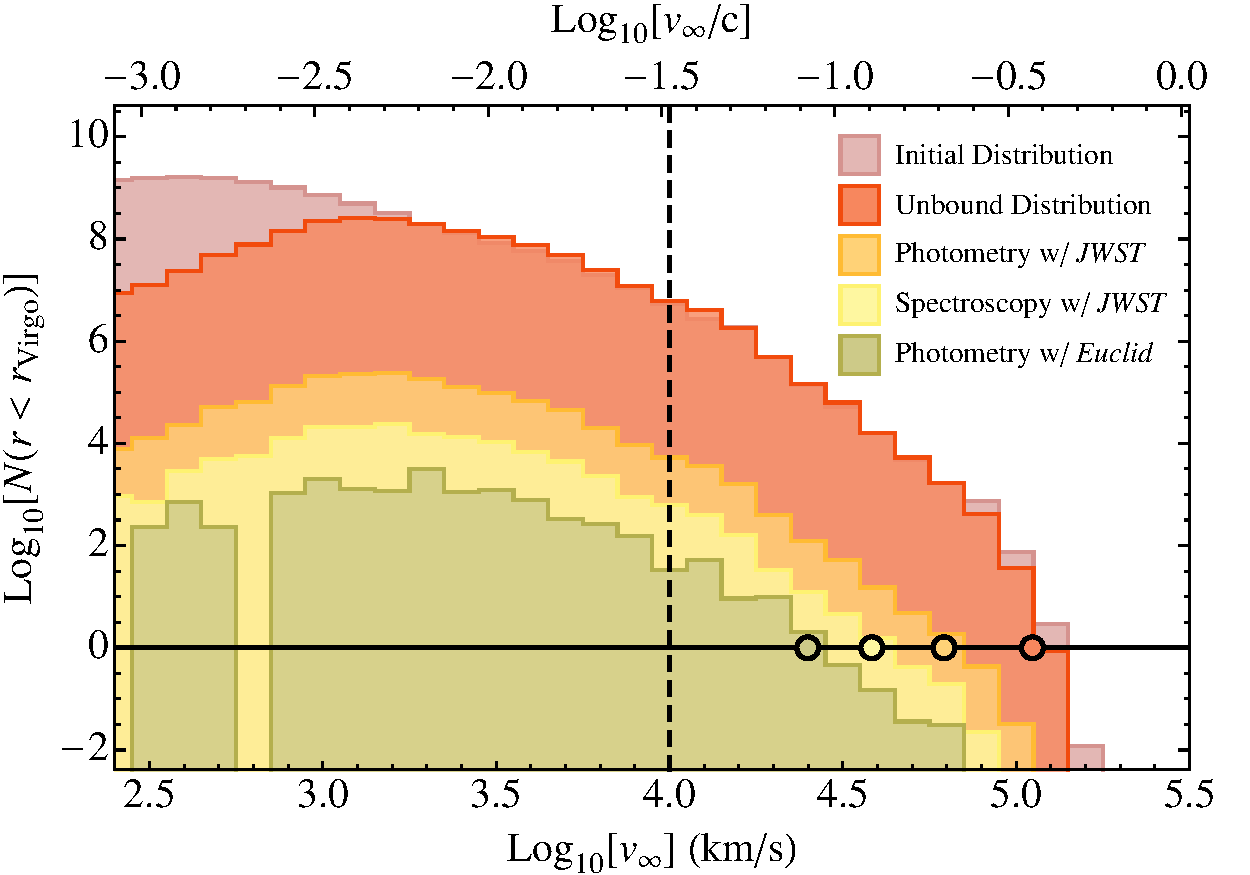
\includegraphics[width=0.7\linewidth,clip=true]{histogram-2}
\caption{Number of SHS satisfying various criteria at a distance $r$ less than that to the Virgo cluster ($r_{\rm Virgo} \simeq 16$ Mpc). The pink histogram shows the initial distribution of SHS resulting from MBH mergers, and only considers the gravitational influence of the black holes themselves. The orange histogram shows the population of unbound SHS after accounting for the fraction of SHS that do not move fast enough to escape their host haloes, resulting in a significant depletion of SHS for \smash{$v_{\infty} \lesssim 10^{3}$ km/s}. Of the SHS that are produced, only a small fraction are bright giants that can be studied with JWST; those that are bright enough to be detected photometrically with NIRCam are shown by the light orange histogram, whereas those stars that are bright enough such that their continuua are detectable by NIRSpec are shown by the yellow histogram. The vertical dashed black line shows $v_{\infty} = 10^{4}$ km/s, the speed limit for the traditional HVS mechanism, all objects to the right of this line can only be produced by merging MBHs. The solid black line shows where the number count is order unity, the colored points along this line show where each distribution crosses this threshold. These intersections suggest that the fastest star in the volume out to Virgo likely travels with $v_{\infty} \simeq$~110,000~km/s, the fastest star detectable with {\it JWST} travels with $v_{\infty} \simeq$~44,000~km/s, the fastest star for which {\it JWST} spectroscopy is possible travels with $v_{\infty} \simeq$~36,000~km/s, and the fastest star likely to be detected with {\it Euclid/WFIRST} travels at 25,000~km/s.}
\label{fig:histogram2}
\end{figure*}

\begin{figure}
\centering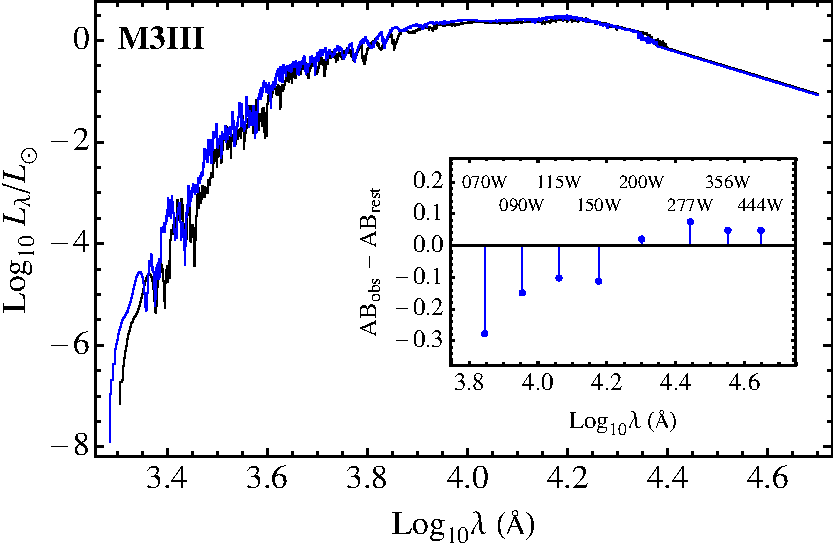
\includegraphics[width=0.9\linewidth,clip=true]{spec-m3iii}
\centering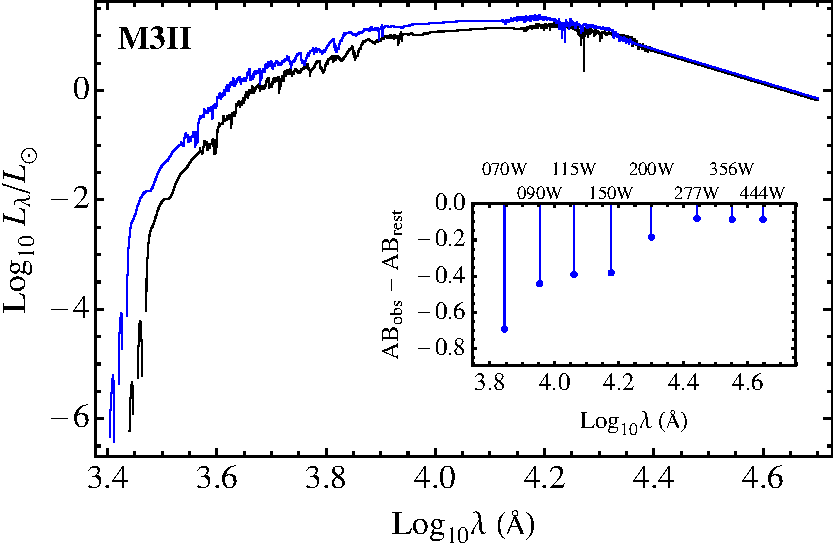
\includegraphics[width=0.9\linewidth,clip=true]{spec-m3ii}\\
\centering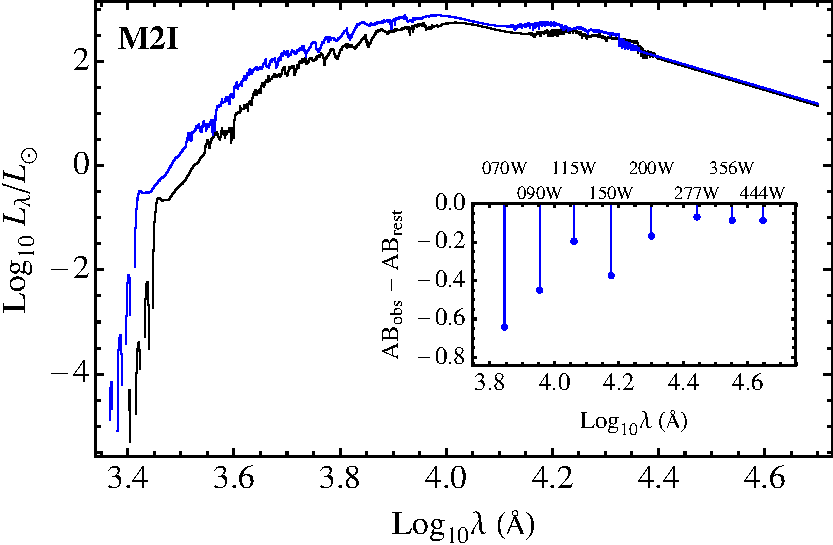
\includegraphics[width=0.9\linewidth,clip=true]{spec-m2i}\\
\caption{Comparisson of rest-frame red giant spectra to blueshifted spectra corresponding to the fastest star likely to be detected by Euclid/WFIRST, $v_{\infty} = 0.08c \simeq$~24,000 km s\smash{$^{-1}$}. Spectra are drawn from the publically available library of \citet{Pickles:1998a}, with the top panel showing an M3III giant, the middle panel showing a M3II giant, and the bottom panel showing an M2I supergiant. As the input spectra only extend to \smash{25,000~\AA}, flux redward of this value are extrapolated assuming a Rayleigh-Jeans law. Inset within each figure is the difference between the observed AB magnitude AB$_{\rm obs}$ for individual {\it JWST} filters versus the magnitude AB$_{\rm rest}$ that would be observed if the star were at rest.}
\label{fig:specs}
\end{figure}

Brief summary: Proper motions in general too small, need nearly all-sky IR survey with limiting magnitude ~24 to detect them. Spectroscopic follow-up with JWST, HST marginal.

HETDEX - Not enough sky coverage, limiting magnitude not good enough ($\sim 20$).

Euclid/WFIRST - All-sky IR surveys, less sensitive than JWST, can detect thousands.

LSST - Fastest stars will tend to be Mpc away and will have little proper motion. May be possible for a small subsample of slower stars, but easily confused with MW sources.

JWST/E-ELT/GMT - Capable of detecting a great number, but limited sky coverage limits the total number that will be detect. All could be used for spectroscopic follow-up.

\section{Avi's relativity calculations}
\colr{Include Avi's new stuff}
To leading order, we consider the trajectory of a fast
non-relativistic star, that reached the vicinity of the Milky-Way
galaxy at the present time $t$ with a measured 3D speed $v_0$. It is
well-known that the peculiar momentum of an object relative to the
Hubble flow, declines inversely with the scale-factor
$a(t)=(1+z)^{-1}$ in an expanding universe\footnote{Naturally, this
implies that the de Broglie wavelength of the particle is stretched by
the sacle factor $a(t)$ like any other physical scale in the expanding
Universe.}. This implies that the peculiar velocity of the star at
earlier times $t<t_0$ was 
\begin{equation}
v=v_0/a(t).
\label{eq:1}
\end{equation}

We assume a flat universe with the metric,
$ds^2=c^2dt^2-a^2(t)(dr^2+r^2d\Omega$, where $r$ is the comoving
(present-day) radius relative to the observer. For simplicity, we
consider the case where the source galaxy from where the star was
ejected at time $t_{ej}$ is much farther away than the distance of the
star from the observer. In that case, the trajectory of the star is
nearly radial towards us, with $v=a(t)dr/dt$. Using Eq. (\ref{eq:1})
we get $dr=v_0 dt/a^2(t)$, and by integrating both sides of this
equation,
\begin{equation}
r(t_{ej})=v_0 \int_{t_{ej}}^{t_0} {dt \over a^2(t)} .
\label{eq:2}
\end{equation}

If the star was ejected when it was much younger than its present age,
$t_\star$, then one could infer $t_{ej}=t_0-t_\star$ from a
spectroscopic measurement of $t_\star$. 

By identifying the source galaxy from the flight time of the star
$t_{star}$ and its spectroscopically inferred radial velocity $v_0$,
one can measure the spectrum of the host galaxy and determine its
redshift $z$. Note that the evolution of $a(t)=(1+z)^{-1}$ depends on
cosmological parameters through the cosmological Friedman equation. In
principle, if the measurement accuracy is sufficiently high, one could
constrain the cosmological parameters (such as the equation of state
of dark matter) by requiring that the source redshift as measured with
photons at $t_0$ would give the correct comoving distance $r(t_{ej})$
for the flight time of a non-relativistic star, according to
Eq. (\ref{eq:2}). Of course, the photons were emitted after the star
left the galaxy, so that they would arrive to us at the same time. In
this context one compare the scale factor when photons were emitted
with the travel time of a non-relativistic star from the same
source. This provides an interesting new variant of the conventional
``Hubble Diagram'' which uses only information gathered by measuring
photons. Such a measurement constitutes a novel test of General
Relativity and the standard model of cosmology.

If the source galaxy is far away, this implies that the star and
galaxy nearly overlap on the sky, although the proper motion of the
star can be used to pinpoint the parent galaxy more accurately. In
case of an overlap, one would need to disentangle the spectral lines
of the two sources (star $+$ galaxy).

\section{Discussion}\label{sec:discussion}
\subsection{Complications}

\begin{figure}
\centering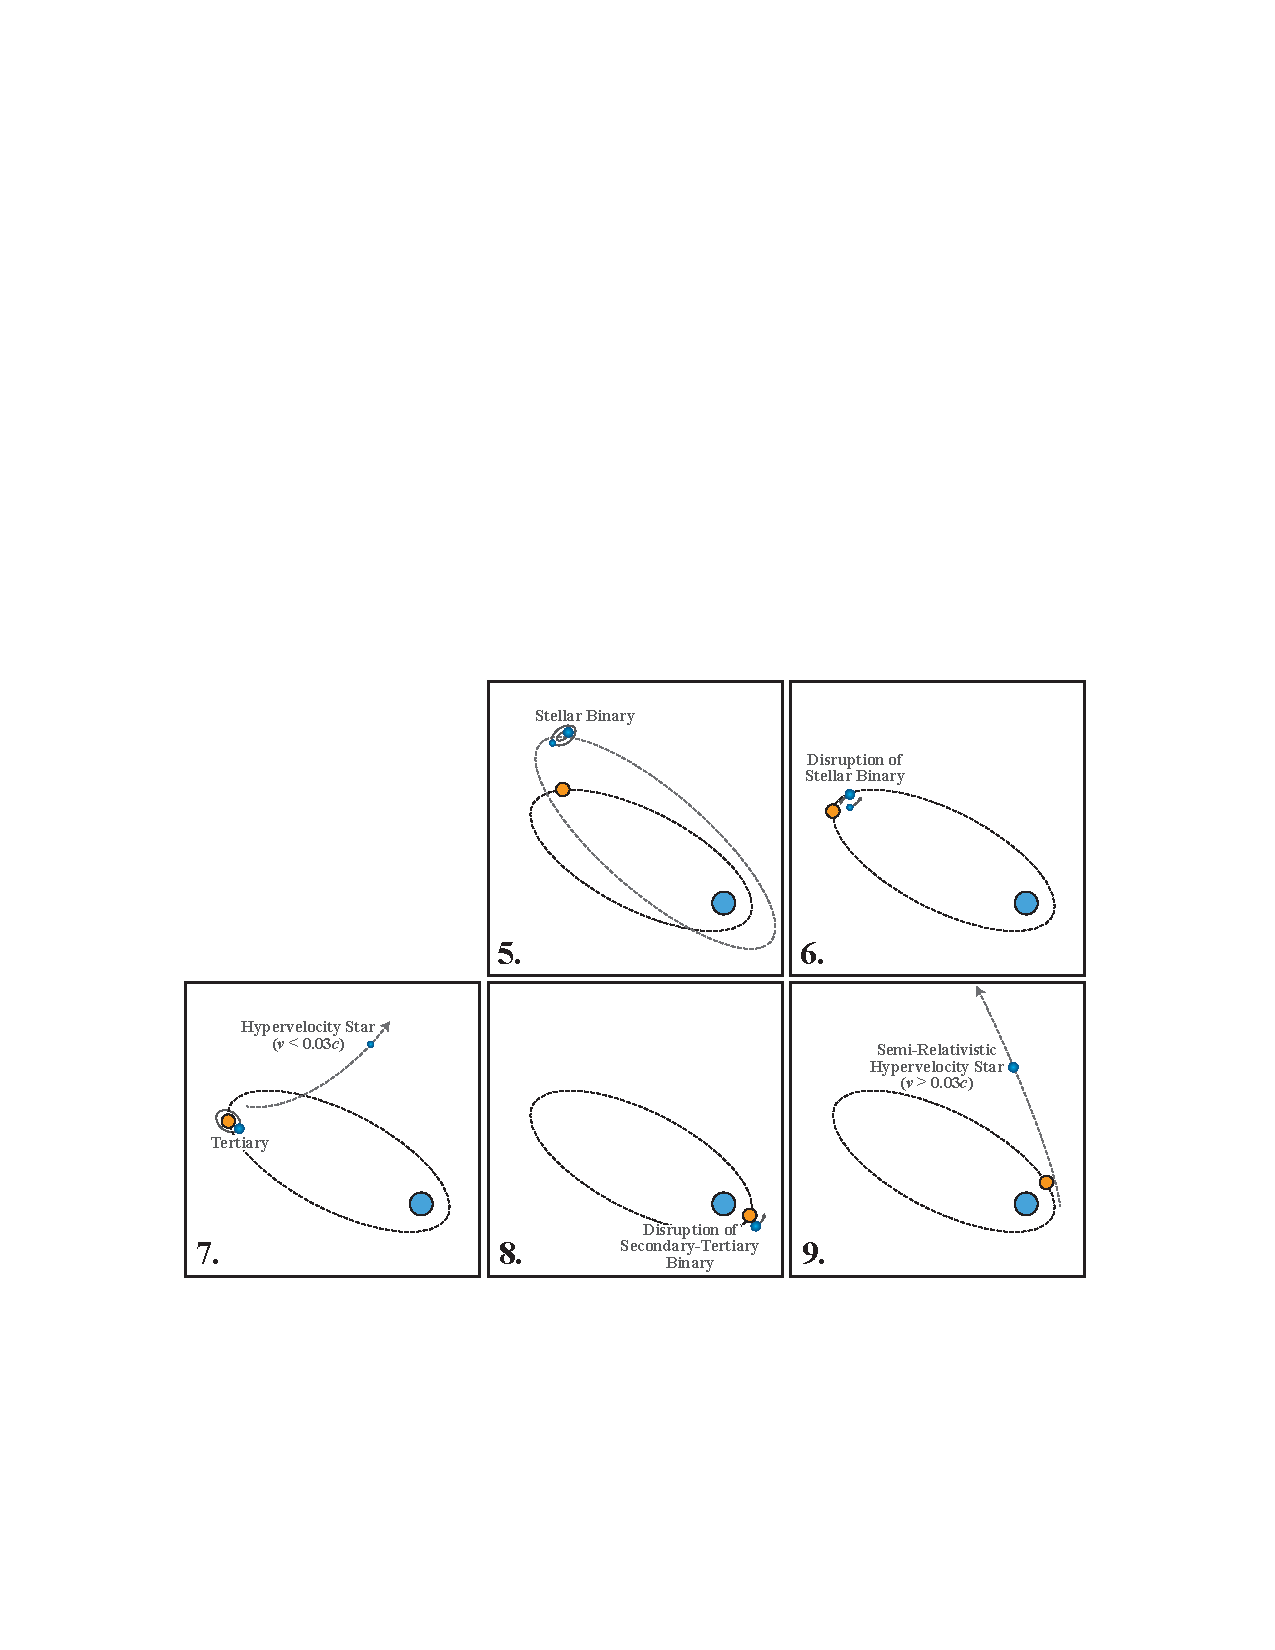
\includegraphics[width=\linewidth,clip=true]{shs-diagram2}
\caption{\colr{Maybe eliminate this figure} Diagram of alternative production channel for SHS. 5: Once the cluster about the secondary is exhausted of its original retinue of stars, a new source of stars is necessary. One possibility is capturing stars via the Hills mechanism from binaries that originally orbit the primary. 6: These binaries pass within their tidal radii with respect to the secondary, resulting in its disruption. 7: One of the two stars is ejected as a hypervelocity star, while the other star (now known as the "tertiary") is retained by the secondary. 8: The secondary-tertiary binary system passes within its tidal radius about the primary, resulting in its disruption. 9: The tertiary is ejected at semi-relativistic speeds, becoming an SHS.}
\label{fig:diagram2}
\end{figure}

\begin{itemize}
\item Near-equal-mass mergers may not have eccentricities driven to $\sim 0.7$, although the critical mass ratio for which eccentricities can be driven to large values is unknown. This also depends sensitively on whether stars are counter- or co-rotating with the black hole's orbit, which can damp eccentricity significantly if a significant fraction of stars co-rotate with the secondary \citep{Sesana:2011a}.
\item Low mass-ratio encounters would have non-plunging orbits, perhaps leading to removal of stars at larger distances, resulting in lower velocities.
\item Eccentricities may not always increase, depending on rotation of cluster surrounding $M_{1}$ \citep{Dotti:2012a}.
\item Collisions may remove stars, also the Schwarzschild barrier may prevent stars from being very close in (read Hamers 2014).
\end{itemize}

\subsection{Implications of a discovery}
As described in \colr{previous section}, stars that are accelerated to speeds in excess of $10^{4}$ km/s are difficult (if not impossible) to produce via any other astrophysical mechanism. Because such large velocities are contingent upon merging supermassive black holes possessing large eccentricities, the discovery of even one SHS would suggest that eccentric MBH mergers are ubiquitous.

\subsection{Scientific Value}
Once identified, a SHS can provide information about matter in distant regions of the universe, where in principle the fundamental constants may vary. The faster the velocity of the discovered star, the more distant its origin (on average), with stars traveling at $c/10$ originating from galaxies that are $\lesssim 1$ Gpc away ($z \sim 0.08$), and stars traveling at $c/2$ originating from galaxies that are $\lesssim 5$ Gpc away ($z \sim 0.5$), assuming both are emitted at $z = 2$.

The baryons in the distant universe are studied by considering the total light produced by galaxies which may contain $\sim 10^{11}$ stars, which requires detailed modeling of their underlying stellar populations to understand the features of its constituent stars. The discovery of an SHS would enable the direct study of a single star that formed in a part of the universe that is now distant to us. 

\section{Outline}
\subsection{To do list}
\begin{itemize}
\item Think about color/flux/prop. motion parameter space, are SHS unique?
\item Show histograms when $q$ cutoffs are included.
\item Mention WFIRST/Euclid together always
\item Run test scattering experiment where $r_{t} = r_{s} = 0$.
\end{itemize}

\subsection{Text}

\begin{itemize}
\item Example disruptions
\item Histograms as functions of velocity
\item Conditions for producing
\item Examples: OJ 287, M87
%We show that the prototypical OJ 287 system, which may be an eccentric MBH binary in the final stages of a merger, is conducive to frequent ejections of such stars because of its tidal capture of stars from binaries originally orbiting the primary. We calculate that this system may have ejected as many as $10^4$ SHS since entering the gravitational wave stage of its merger. 
\item Iwasawa driving eccentricity
\item Estimate of co-moving density
\item Cosmological context
\item Detection with JWST, HST, LSST, EELT, GMT, TMT, Euclid, WFIRST
\item -- Measurement of proper motion
\item -- Velocity
\item -- Age
\item Test the equivalence principle
\item Way to identify LISA sources
\end{itemize}

Additional Notes: Anne-Marie Madigan paper suggested by Cole Miller on eccentricity damping of MBH binaries.

\subsection{Figures}
\begin{enumerate}
\item Histogram of velocities/distance
\item Collage of fast stars
\item Number of stars as function of flux for different velocity bins
\end{enumerate}

\acknowledgements
We acknowledge K. Batygin, P. Groot, M. Holman, S. Naoz, A. Sesana, Y. Levin. We are especially grateful to M. C. Miller for extended discussions regarding the mechanism presented here.

\bibliographystyle{apj}
\bibliography{/Users/james/Dropbox/library}

\end{document}

